The Proper Generalized Decomposition (PGD) is a technique to efficiently solve a multidimensional problem. It relies on progressive enrichments performed not on each individual case of the problem, but on the structure of the problem as a whole \cite{chinesta2010recent,blanco2017efficient}. The outcome of the PGD becomes a potentially well-refined solution for various scenarios that have not been computed directly. Indeed, this comes with an associated saving of time. 

Backed by its mathematical proof, this chapter presents the notation, the definitions of the objects, and more importantly, a practical algorithm overview.

\subsection{Derivation}
It is a well-known fact that the power flow problem is mainly concerned with four magnitudes: voltages denoted by $\bm{V}$, currents represented by $\bm{I}$, complex powers given by $\bm{S}$ and the bus admittance matrix $\bm{Y}$. The usage of bold variables indicates that these are multidimensional objects.

The first novelty of the PGD has to do with their tensorial representation. This arises from the crossing of multiple vectors, each describing a dimension of the form 
\begin{equation}
	\bm{Z} (\bm{x},\bm{t},\bm{p_1},\bm{p_2},...,\bm{p_D}) = \sum_{i=1}^{n}X(\bm{x})\otimes T(\bm{t})\otimes P_1(\bm{p_1})\otimes P_2(\bm{p_2})\otimes ... \otimes P_D(\bm{p_D}) \ ,
\label{eq:full}
\end{equation}
where $\bm{Z}$ represents either $\bm{V}$, $\bm{I}$ or $\bm{S}$. Note the dependence on position ($\bm{x}$), time ($\bm{t}$) and the parameters meant to change ($\bm{p_1}$ to $\bm{p_D}$). In the power flow problem, $\bm{x}$ stands for the indices attributed to the buses while the parameters can be for instance variations in power in several buses. Changes in impedance could also be parametrized, although it is not clear how the PGD should be adapted to it. Notice also that the final tensor is the result of the sum of multiple tensors with the same dimensions. One tensor could represent the stationary power we predict, while another one could be the variations we introduce, for instance.

Recall that by definition solving the power flow means solving
\begin{equation}
\bm{Y}\bm{V}=\frac{\bm{S^*}}{\bm{V^*}} \ ,
\label{eq:YV0}
\end{equation}
for $\bm{V}$. Considering the presence of a slack bus, where the voltage is already known and its current injection to the rest of the buses is symbolized by $\bm{I_0}$, Equation \ref{eq:YV0} becomes
\begin{equation}
\bm{YV} = \bm{I_0} + \bm{\frac{S^*}{V^*}} \ .
\label{eq:YV}
\end{equation}
which translates into the following in compact form
\begin{equation}
	\bm{V} = \bm{Y^{-1}}(\bm{I_0}+\bm{S^*}\oslash\bm{V}) \ ,
\label{eq:V1}
\end{equation}
where $\oslash$ denotes the Hadamard division, that is, the element-wise division. As described in \cite{garcia2016reduced}, the power flow problem can be solved with the so-called alternating search directions (ASD) method. This has the advantage of combining quite adequately with the PGD methodology due to its speed, but mainly, because of the linear relationship between voltages and currents during one of the two steps in which the PGD is divided. 

The two steps we are referring to are first of all the non-linear connection between voltages and currents
\begin{equation}
	\bm{I}=\bm{S^*}\oslash \bm{V^{*[\gamma]}} \ .
\label{eq:In}
\end{equation}
where $\gamma$ indicates the outer loop iteration number. Here the variables are in fact tensors. Note that the traditional way to solve Equation \ref{eq:In} would be to compute all the cases, one by one. However, this is not beneficial and it is not the point of the PGD. In fact, the PGD circumvents this problem. 

The second step to perform is described by 
\begin{equation}
	\bm{V^{[\gamma+1]}} = \bm{Y^{-1}}(\bm{I}+\bm{I_0}) \ .
\label{eq:Vg1}
\end{equation}
The procedure consists of first computing $\bm{I}$ from Equation \ref{eq:In} using the PGD method. Once this is done, we proceed to update $\bm{V}$. In the end, it follows the same structure as $\bm{I}$ because they are related by a linear transformation, which saves computation time.

The complexity of solving this problem lies in Equation \ref{eq:In}. The second step given by Equation \ref{eq:Vg1} is direct. Recall that the tensor $\bm{Z}$ shown in Equation \ref{eq:full} represents in a general form $\bm{S}$, $\bm{V}$ and $\bm{I}$. Hence, we define $\bm{u^T}\bm{V^*}\bm{I} = \bm{u^T}\bm{S^*}$, where the superscript $T$ stands for the transposed operation. The redefinition of $\bm{I}$ is
\begin{equation}
	\bm{I}=\sum_{i=1}^{n}\bm{i_1}\otimes \bm{i_2} \otimes ... \otimes \bm{i_D} + \bm{R_1}\otimes ... \otimes \bm{R_D} \ .
\label{eq:decomp}
\end{equation}
The so-called test field follows 
\begin{equation}
\bm{u} = \bm{R_1}^*\otimes \bm{R_2} \otimes ... \otimes \bm{R_D} + ... + \bm{R_1}\otimes \bm{R_2} \otimes ... \otimes \bm{R_D}^* \ .
\label{eq:decomp2}
\end{equation}
This implies the following, in extended form:
\begin{equation}
	\begin{split}
		\sum_{i=1}^{N_v}\sum_{j=1}^{n} & \bm{R_1^{T*} V_1^{i*} i_{1}^{j}} \times ... \times \bm{R_D^{T}V_D^{i*}i_D^j }  + ... + \sum_{i=1}^{N_v}\sum_{j=1}^{n}\bm{R_1^{T} V_1^{i*} i_{1}^{j}} \times ... \times  \bm{R_D^{T*}V_D^{i*}i_D^j } \\
					       & + \sum_{i=1}^{N_v}\bm{R_1^{T*}V_1^{i*}R_1} \times ... \times \bm{R_D^{T}V_D^{i*} R_D } + ... + \sum_{i=1}^{N_v}\bm{R_1^{T}V_1^{i*}R_1} \times ... \times \bm{R_D^{T*}V_D^{i*} R_D } = \\
					       & \sum_{i=1}^{N_s}\left(\bm{R_1^{T*}S_1^{i*}}\times ... \times \bm{R_D^T S_D^{i*}} + ... + \bm{R_1^T S_1^{i*}} \times ... \times \bm{R_D^{T*}S_D^{i*}}\right) \ . 
		\end{split}
\label{eq:full2}
\end{equation}
Which can be compacted by defining 
\begin{equation}
	\sum_{i=1}^{N_c}\bm{C_1^i}\otimes ... \otimes \bm{C_D^i} = \sum_{i=1}^{N_s}\bm{S_1^{i*}}\otimes ... \otimes \bm{S_D^{i*}} - \sum_{i=1}^{N_v}\sum_{j=1}^n \bm{V_1^{i*}i_1^{j}}\otimes ... \otimes \bm{V_D^{i*}i_D^{j}} ,
\label{eq:full3}
\end{equation}
where $N_c=N_s + N_vn$. This way, the problem described by Equation \ref{eq:full2} takes the form of 
\begin{equation}
	\begin{split}
		\sum_{i=1}^{N_v}& \bm{R_1^{T*}V_1^{i*}R_1} \times ... \times \bm{R_D^{T}V_D^{i*} R_D } + ... + \sum_{i=1}^{N_v}\bm{R_1^{T}V_1^{i*}R_1} \times ... \times \bm{R_D^{T*}V_D^{i*} R_D } = \\
				& \left(\bm{R_1^{T*}}\otimes ... \otimes \bm{R_D^{T}} + ... + \bm{R_1^T}\otimes ... \otimes \bm{R_D^{T*}}  \right)	\sum_{i=1}^{N_c}\bm{C_1^i}\otimes ... \otimes \bm{C_D^i} \ .
	\end{split}
\label{eq:full4}
\end{equation}
At this stage, a greedy algorithm is implemented \cite{black2005greedy}. This technique serves the purpose to find the multiple $\bm{R_i^{[\Gamma]}}$ for $i=1,...,D$, where $\Gamma$ represents the iteration number of this inner loop. This way, there are three loops. The outer one is the ASD as such, that is, the algorithm responsible for solving the power flow problem. The intermediate one deals with finding the residues at every superposition of the $\bm{I}$ tensor. To do so, the last and most inner loop is the one that goes over the several $\Gamma$ indices to iterate and find convenient residues. This can be summarized by:
\begin{itemize}
	\item Outer loop: iterate on $\gamma$ to solve the power flow as such.
	\item Intermediate loop: iterate on $i$ to find the superposition of terms of the  $\bm{I}$ tensor.
	\item Inner loop: iterate on $\Gamma$ to find the residues $\bm{R_k^{\Gamma}}\forall k \in [1,...,D]$.
\end{itemize}

Finally, the residues of the form $\bm{R_k^{\Gamma}}$ are computed with
\begin{equation}
	\left(\sum_{i=1}^{N_v}\bm{V_k^{i*}}\prod_{j\neq k}^D \bm{R_j^TV_j^{i*}R_j}\right)\bm{R_k} = \sum_{i=1}^{N_c}\bm{C_k^i}\prod_{j\neq k}^D\bm{R_j^TC_j^i} \ .
\label{eq:residue1}
\end{equation}
Once this is done for all residuals $k$, an inner iteration $\Gamma$ has finished. Note that the superscript $\Gamma$ has been avoided in Equation \ref{eq:residue1} to alleviate the notation. But the point is that $\bm{R_k}$ is computed from the previously known residues, which are also going to be updated. In essence, this replicates the Gauss-Seidel method. It is recommended to iterate several times in this inner loop to refine the solution. Usually, around 10 to 20 times is more than enough. The same applies to the intermediate loop, where the number of iterations can change at each step according to the necessities. That is, the parameter $M$ is arbitrary and can change from time to time \cite{garcia2016reduced}. Once $\bm{I}$ is fully built, the voltages are updated and the iteration procedure continues until a satisfactory solution has been generated.

\subsection{Application}
The steps involved in the PGD are schematically shown in Algorithm \ref{alg:seq} for a generic case with arbitrary parameters.

\begin{algorithm}[H]
\begin{algorithmic}[1]
\FOR{$\gamma=1$ to $N_\gamma$}
\STATE Calculate power side of the problem with PGD: $\bm{I}=\bm{S^*} \oslash \bm{V^{*[\gamma]}}$
\FOR{$i=1$ to $n$}
\STATE Define $\bm{I}=\sum_{i=1}^{n-1} \bm{P^{(i)}_1} \otimes \bm{P^{(i)}_2} \otimes ... \otimes \bm{P^{(i)}_{D}} +  \bm{P^{(n)}_1} \otimes \bm{P^{(n)}_2} \otimes ... \otimes \bm{P^{(n)}_{D}} $
\FOR{$\Gamma=1$ to $N_{\Gamma}$}
% 000000000000000000000000
\STATE Compute $\bm{P_1^{(n)[\Gamma+1]}}$ with $\bm{P_2^{(n)[\Gamma]}}$,...,$\bm{P_{D}^{(n)[\Gamma]}}$.   
\STATE Compute $\bm{P_2^{(n)[\Gamma+1]}}$ with $\bm{P_1^{(n)[\Gamma+1]}}$ and $\bm{P_3^{(n)[\Gamma]}}$,...,$\bm{P_{D}^{(n)[\Gamma]}}$.   
\STATE $\vdots$
\STATE Compute $\bm{P_D^{(n)[\Gamma+1]}}$ with $\bm{P_1^{(n)[\Gamma+1]}}$,...,$\bm{P_{D-1}^{(n)[\Gamma+1]}}$.   
\ENDFOR
\ENDFOR
\STATE Calculate admittances side of the problem directly: $\bm{V^{[\gamma+1]}}=\bm{Y^{-1}}(\bm{I}+\bm{I_0})$.
\ENDFOR
\end{algorithmic}
\caption{Pseudocode for the PGD combined with the ASD}
\label{alg:seq}
\end{algorithm}
Solving the power flow for each variation in the parameters with the classical Newton-Raphson is without a doubt more straightforward than following the procedure summarized in Algorithm \ref{alg:seq}. % add the algo!
 The price to pay for this simplicity is in the time required, which in computational terms is usually called complexity. The Newton-Raphson involves at least one inversion of the Jacobian matrix, and usually between three to five in order to obtain results with appropriate precision. It is a well-known fact that the complexity of a $n \times n$ inverse matrix increases exponentially with its size \cite{he2009research}, and in principle, it is $\mathcal{O}(n^3)$. Therefore, having to compute the inverse so many times in power flow problems where parameters change slightly becomes an arduous task. 

On the contrary, the PGD becomes a much more efficient methodology. There are no inverse matrices involved (apart from the impedance matrix, which can be precomputed) and it is able to decouple the dimensions of the problem. Take for instance a system where three parameters $p_1$, $p_2$ and $p_3$ vary in ranges of $n_1$, $n_2$ and $n_3$ values. If the total number of non-slack buses in the system is $n_b$, the amount of calculations $N_u$ turns out to be
\begin{equation}
   N_u \propto M (n_b + n_1 + n_2 + n_3) \ ,
\label{eq:n_unk_pgd}
\end{equation}
where $M$ is the so-called number of modes and corresponds to the number of iterations performed in the intermediate loop. Instead, a Newton-Raphson-based algorithm would require to compute $N_r$ unknowns, where 
\begin{equation}
   N_r \propto n_bn_1n_2n_3  \ .
\label{eq:n_unk_nr}
\end{equation}
When the dimensions of the system tend to large values, the PGD becomes considerably faster than the Newton-Raphson. For example, \cite{blanco2017efficient} reported solving in a matter of minutes a time-series power flow which took a couple of hours with the Newton-Raphson method.  

Leaving aside the mathematical formulation, we introduce a basic example to illustrate the dimensionally of the power flow problem in a renewable penetration scenario. Figure \ref{fig:3xp_2} shows how the total power $P$ changes according to the demand of power $P_d(t)$ and the power generated from hypothetical windmills, denoted by $P_g(v_w)$. Thus, the variables involved are the time $t$ and the wind speed $v_w$. The total power has been defined as $P=P_d(t)-P_g(v_w)$, which can be understood as a net balance of the demand, and for convenience it is expressed as an adimensional quantity.

% \pgfplotsset{
% colormap={whitered}{color(0cm)=(white!95!orange); color(1cm)=(orange!75!red)}
% }

\pgfplotsset{
colormap={whitered}{color(0cm)=(white!95!black); color(1cm)=(gray!85!black)}
}

\begin{figure}[!htb]\centering
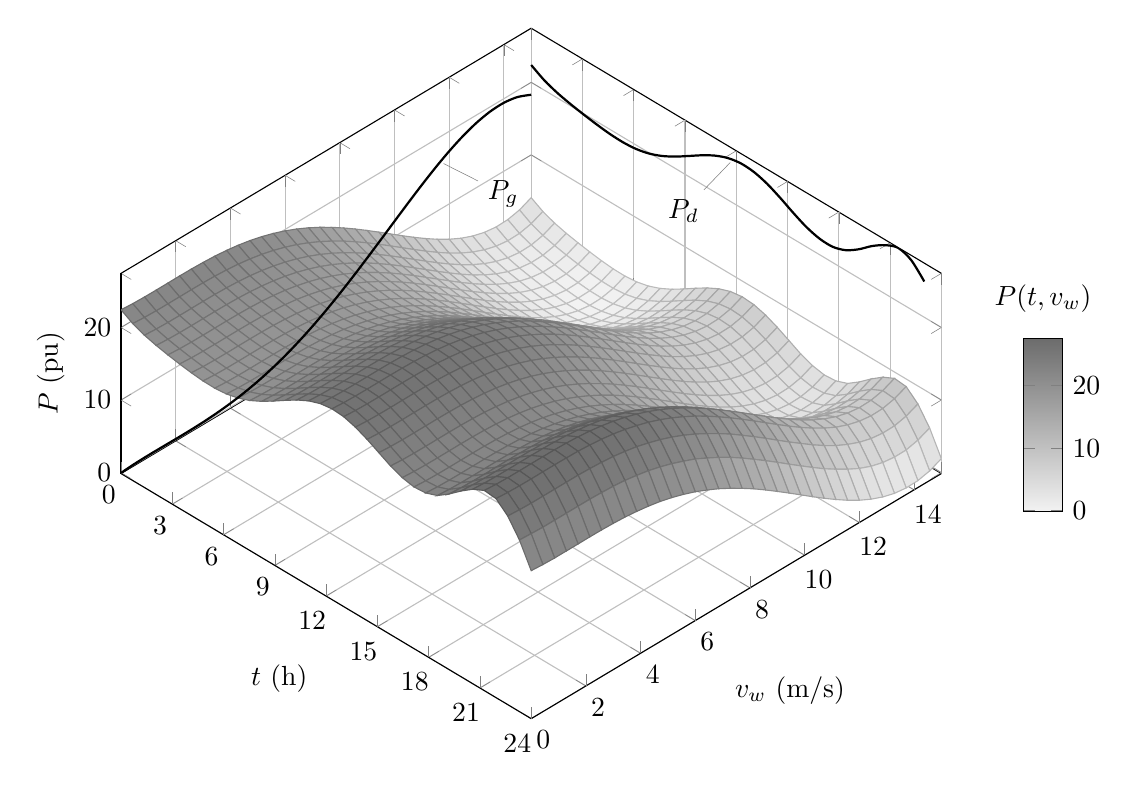
\begin{tikzpicture}[
  declare function = {mu1=1;},
  declare function = {mu2=2;},
  declare function = {sigma1=0.5;},
  declare function = {sigma2=1;},
  declare function = {normal(\m,\s)=1/(2*\s*sqrt(pi))*exp(-(x-\m)^2/(2*\s^2));},
  declare function = {bivar(\ma,\sa,\mb,\sb)=
    1/(2*pi*\sa*\sb) * exp(-((x-\ma)^2/\sa^2 + (y-\mb)^2/\sb^2))/2;},
  declare function = {Pwind(\x)=  -0.04848479278074868 + 0.3828985204520174*\x  - 0.2608981245129764*\x*\x + 0.061004598841255586*\x*\x*\x - 0.002658684188611232 *\x*\x*\x*\x ;},
  declare function = {Pdemand(\y)=  22.394708020782733 - 1.6354720294954328*\x + 0.39434274588533585*\x*\x - 0.0035090092967717756*\x*\x*\x - 0.029337034458808153*\x*\x*\x*\x + 0.007731225380636515*\x*\x*\x*\x*\x - 0.0008557978395676469*\x*\x*\x*\x*\x*\x + 0.00004732882729208937 *\x*\x*\x*\x*\x*\x*\x - 0.00000128996363643316*\x*\x*\x*\x*\x*\x*\x*\x + 1.381540655448e-8*\x*\x*\x*\x*\x*\x*\x*\x*\x ;},
  declare function = {Ptotal(\x,\y) = -(1.6349 - 10.719343177393107*\x + 11.204527200243698 *\x*\x - 2.55136190066593*\x*\x*\x + 0.17642202760515993*\x*\x*\x*\x) + 22.394708020782733 - 1.6354720294954328*\x + 0.39434274588533585*\x*\x - 0.0035090092967717756*\x*\x*\x - 0.029337034458808153*\x*\x*\x*\x + 0.007731225380636515*\x*\x*\x*\x*\x - 0.0008557978395676469*\x*\x*\x*\x*\x*\x + 0.00004732882729208937 *\x*\x*\x*\x*\x*\x*\x - 0.00000128996363643316*\x*\x*\x*\x*\x*\x*\x*\x + 1.381540655448e-8*\x*\x*\x*\x*\x*\x*\x*\x*\x ;},
  declare function = {P1(\a) = -0.04848479278074868 + 0.3828985204520174*x  - 0.2608981245129764*x*x + 0.061004598841255586*x*x*x - 0.002658684188611232 *x*x*x*x + 0.00001*\a ;},
  declare function = {P2(\b) = + 22.394708020782733 - 1.6354720294954328*x + 0.39434274588533585*x*x - 0.0035090092967717756*x*x*x - 0.029337034458808153*x*x*x*x + 0.007731225380636515*x*x*x*x*x - 0.0008557978395676469*x*x*x*x*x*x + 0.00004732882729208937*x*x*x*x*x*x*x - 0.00000128996363643316*x*x*x*x*x*x*x*x + 0.00000001381540655448*x*x*x*x*x*x*x*x*x + 0.00001*\b ;},
  declare function = {P3(\c) = - ( -0.04848479278074868 + 0.3828985204520174*y  - 0.2608981245129764*y*y + 0.061004598841255586*y*y*y - 0.002658684188611232 *y*y*y*y ) + 22.394708020782733 - 1.6354720294954328*x + 0.39434274588533585*x*x - 0.0035090092967717756*x*x*x - 0.029337034458808153*x*x*x*x + 0.007731225380636515*x*x*x*x*x - 0.0008557978395676469*x*x*x*x*x*x + 0.00004732882729208937*x*x*x*x*x*x*x - 0.00000128996363643316*x*x*x*x*x*x*x*x + 0.00000001381540655448*x*x*x*x*x*x*x*x*x + 0.00001*\c ;}, 
  declare function = {P4(\c) = 0*x + -0.25 + 0.00001*\c ;},
    ]
  \begin{axis}[
    colormap name  = whitered,
    width          = 12cm,
    view           = {45}{60},
    enlargelimits  = false,
    grid           = major,
    domain         = 0:24,
    y domain       = 0:15,
    xtick distance = {3},
    ytick distance = {2},
    samples        = 36,
    xlabel         = $t$ (h),
    ylabel         = $v_w$ (m/s),
    zlabel         = {$P$ (pu)},
    colorbar,
    colorbar style = {
      at     = {(1.1,0.3)},
      anchor = south west,
      height = 0.25*\pgfkeysvalueof{/pgfplots/parent axis height},
      title  = {$P(t,v_w)$}
    }
  ]
    \addplot3 [surf] {P3(1)};
    \addplot3 [domain=0:23,samples=31, samples y=0, thick, smooth]
      (x,15,{P2(1)});
    \addplot3 [domain=0:15,samples=31, samples y=0, thick, smooth]
      (0,x,{P1(1)});

    \node at (5.5,8,33) [pin=-15:$P_g$] {};
    \node at (17,12,41) [pin=-130:$P_d$] {};
  \end{axis}
\end{tikzpicture}
\caption{Evolution of the net power depending on the time of consumption and on the wind speed. Data for the demand curve are extracted from Red Eléctrica de España \cite{ree_demand}.}
  \label{fig:3xp_2}
\end{figure}

If all the possible operating points of the grid have to be assessed, all the combinations of power have to be considered. On the one hand the demand can vary in its typical form, with peaks around mid-day and the evening, and a valley at night. The power generated by a wind power plant is assumed to first follow a cubic evolution and then stabilizes around the nominal power. No cut-out speed has been represented for convenience purposes. In any case, wind can blow at any speed independently of the time of the day. Thus, if all possible operating states have to be studied, one needs to solve the system for each combination. 

There are only two parameters in the situation considered in Figure \ref{fig:3xp_2}, that is, time $t$ and wind speed $v_w$. It is not hard to imagine how an electric system may have more than two parameters. For instance, solar irradiance could also be taken into account, and in addition to that, various places may have different natural resources at the same point in time. So in that regard, conventional power flow strategies would have to compute thousands and thousands of cases. This is of course a non-scalable way to attack the problem. Because of that, we have introduced the PGD as a way to efficiently solve the multidimensional power flow. 
